\documentclass[conference]{IEEEtran}
\usepackage[cmex10]{amsmath}
\usepackage{xcolor}
\usepackage{graphicx}
\hyphenation{op-tical net-works semi-conduc-tor}

\begin{document}
\title{FSK Receiver\\ECE 432 Microwave Circuit Design II}
\author{\IEEEauthorblockN{Jackson Pugh}
\IEEEauthorblockN{Michael Woodruff}
\IEEEauthorblockA{Portland State University\\
Portland, OR 97207}}
\maketitle
\IEEEpeerreviewmaketitle
\section{FSK Receiver Background}

\section{FSK Receiver Design}
The following sections describe the design and building procedures for each part of the FSK receiver.  At the end, the results are documented and analyzed.

\section{LNA Design}
\section{LNA Simulation}
\section{LNA Lab Results}
\section{Wilkinson Divider Design}
The design of the Wilkinson power divider was done with the aid of ADS's built in Wilkinson divider coupler tool\footnote{It is available in the DesignGuide -$>$ Passive Circuit menu.}.  The result can be seen in Figure~\ref{fig:WDSchematic}.  Transmission line was added on the outputs to be able to connect the bandpass filters.  The simulation results, shown in Figure~\ref{fig:WDSim}, gives close to a -3-dB insertion loss for both 2.4 GHz and 2.6 GHz as expected.  Figure~\ref{fig:WDLayout} shows the layout used when manufacturing the board in the EPL.

% WD circuit schematic
\begin{figure}[!htb]
\centering
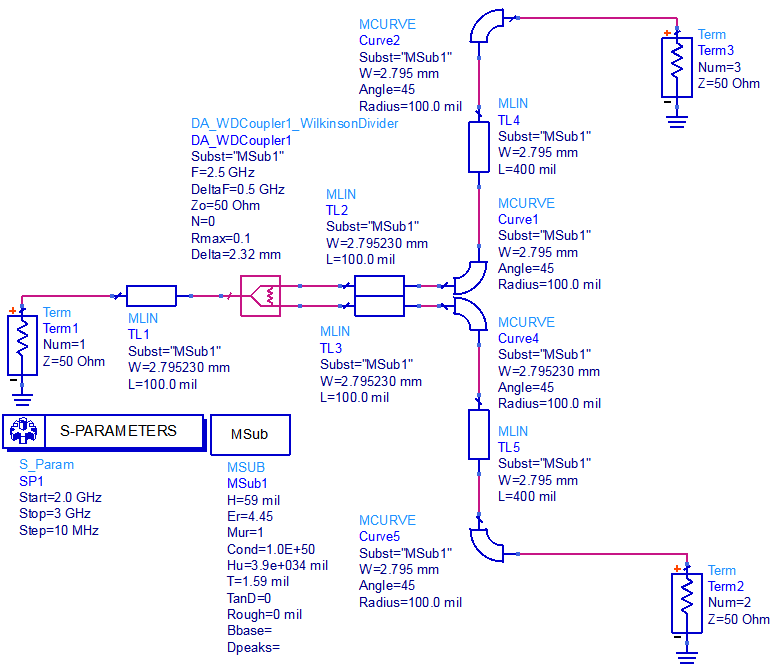
\includegraphics[scale=0.4]{wilkinson-pics/wilkinson-schematic.png}
\caption{Wilkinson power divider schematic.}
\label{fig:WDSchematic}
\end{figure}

% WD simulation
\begin{figure}[!htb]
\centering
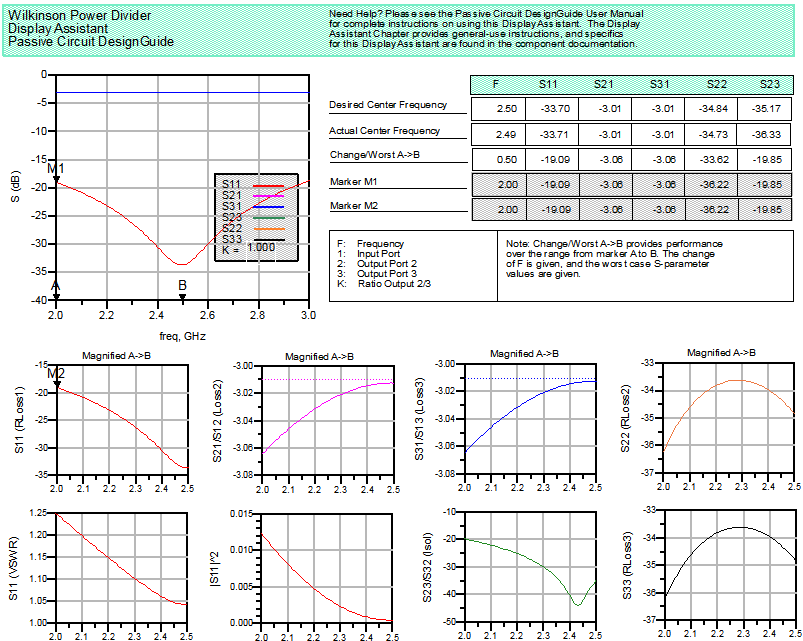
\includegraphics[scale=0.4]{wilkinson-pics/wilkinson-simulation.png}
\caption{Simulation results for the Wilkinson power divider.}
\label{fig:WDSim}
\end{figure}

% WD layout
\begin{figure}[!htb]
\centering
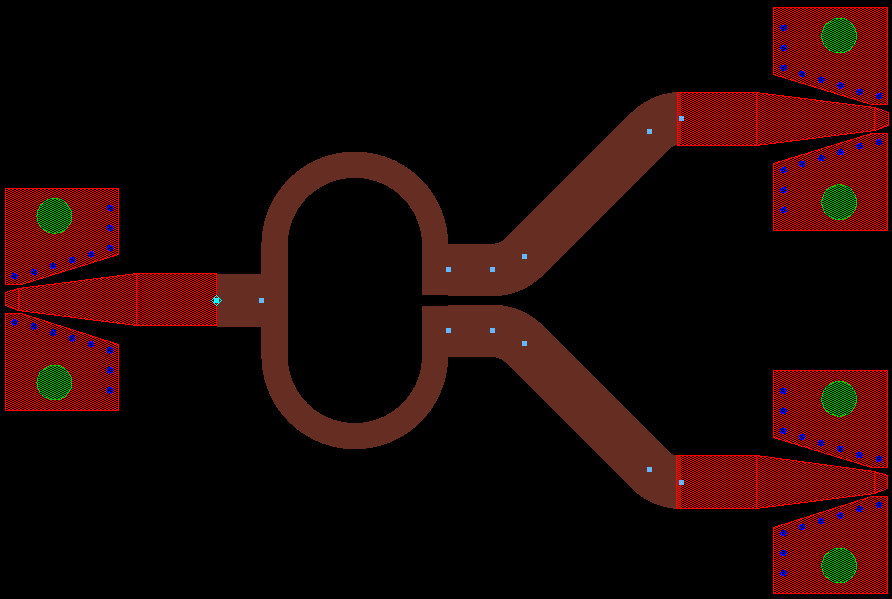
\includegraphics[scale=0.35]{wilkinson-pics/wilkinson-layout.png}
\caption{Wilkinson power divider layout.}
\label{fig:WDLayout}
\end{figure}

\section{Bandpass Filter Lab Results}
The 2.4 GHz and 2.6 GHz bandpass filters were designed by our TA Lunan Zhang\cite{lunan}.  The results for the 2.4 GHz and 2.6 GHz bandpass filter are shown in Figure~\ref{fig:bpf24} and Figure~\ref{fig:bpf26}, respectively.  The filters were off by about 100 MHz and will have an impact on the overall FSK receiver design.

% 2.4 GHz result
\begin{figure}[!htb]
\centering
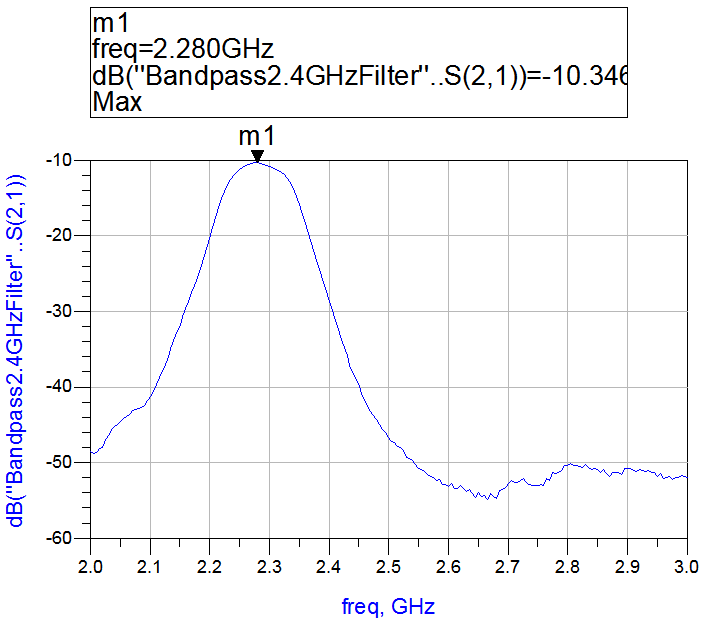
\includegraphics[scale=0.35]{bandpass-pics/bpf24.png}
\caption{Lab result for the 2.4 GHz bandpass filter.}
\label{fig:bpf24}
\end{figure}

% 2.6 GHz result
\begin{figure}[!htb]
\centering
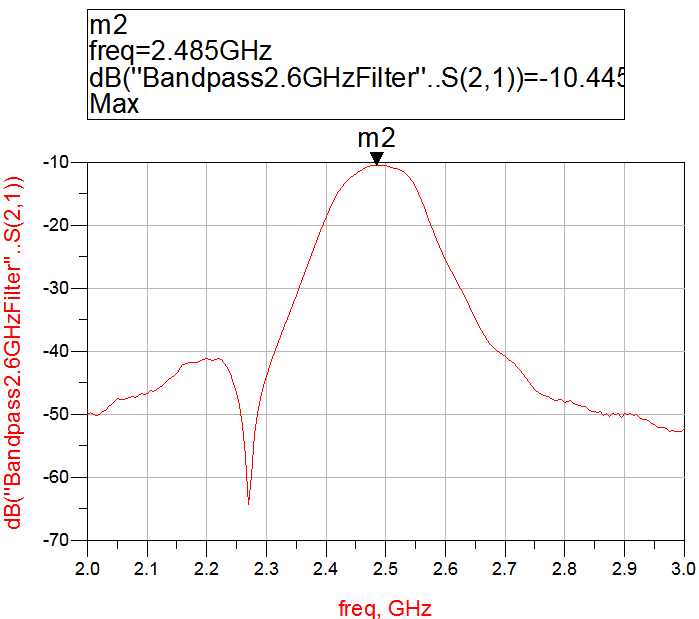
\includegraphics[scale=0.35]{bandpass-pics/bpf26.png}
\caption{Lab result for the 2.6 GHz bandpass filter.}
\label{fig:bpf26}
\end{figure}

\section{Diode Detector Background}
Diode detectors are used to detect if a signal is present.  Matching circuits are often required to detect a specifc frequency.

\section{Diode Detector Design}
The design of the diode detector circuit consisted around the Avago HSMS-2860 Schottky detector diode.  Figure~\ref{fig:DDSchematic} shows a simplified diode detector circuit.  Supporting components including R1, R4, and C4.  R1 and C4 act as a low pass filter to block out high frequencies.  R4 creates the forward diode potential, thus turning the diode on.  A secondary effect R4 imposes on the circuit is it moves the input impedance closer to the origin.  Avago's AN 1124\cite{an1124} was used to properly model the parasitics involved with packaging and wiring the diode detector, which is shown in Figure~\ref{fig:diodeModel}.  In order to detect frequencies at 2.4 and 2.6 GHz, an input matching network will be required.  Figure~\ref{fig:DDPlot} shows the Smith chart plot for the simple diode detector circuit.  In order to properly match for the correct frequencies, a built-in tool provided by ADS will be utilized.  Figure~\ref{fig:smithchartTool} shows the Smith Chart tool that was used to design the input matching network.  Table~\ref{tab:diodetable} shows the final microstrip line lengths.  Tuning was used to obtain the final values.  Figure~\ref{fig:FinalDDSchematic} shows the final circuit schematic.  

% Diode detector simple circuit schematic
\begin{figure}[!htb]
\centering
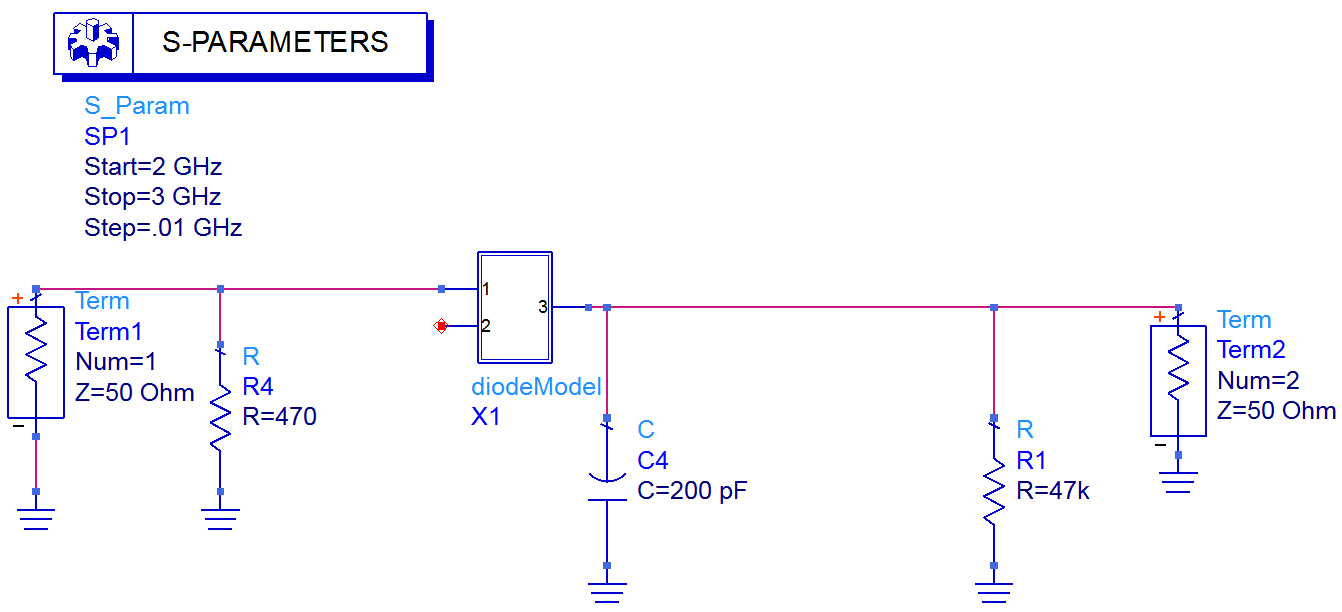
\includegraphics[scale=0.25]{diode-pics/diodedetectorSimplifiedSchematic.png}
\caption{Simple diode detector circuit with unmatched input.}
\label{fig:DDSchematic}
\end{figure}

% Diode Model
\begin{figure}[!htb]
\centering
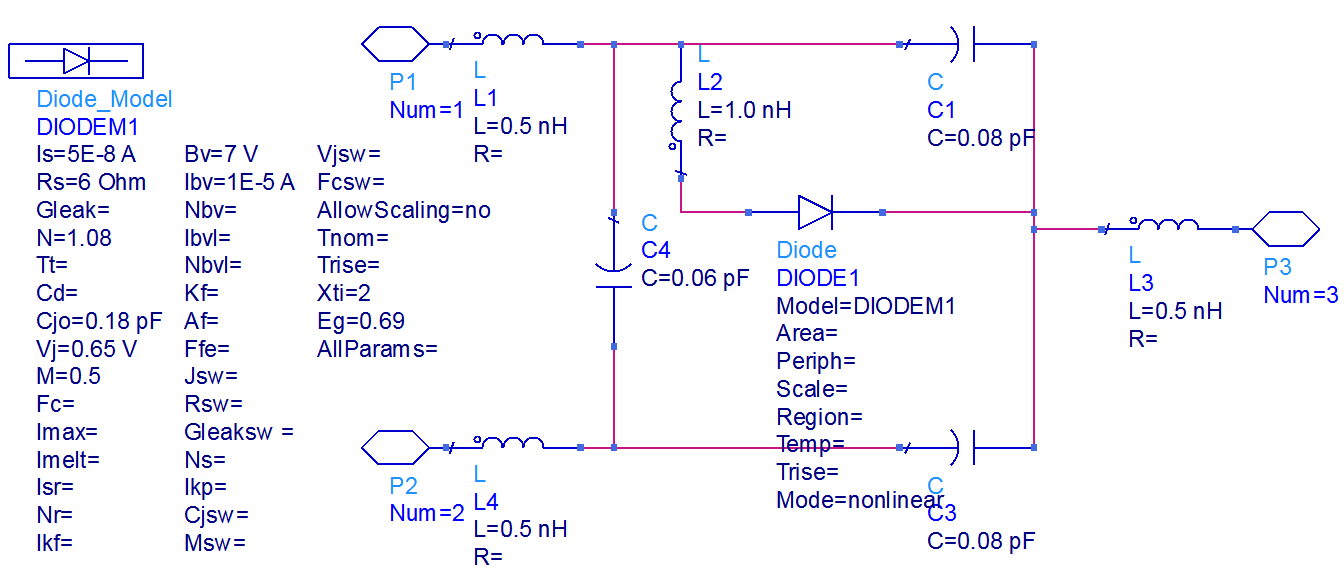
\includegraphics[scale=0.25]{diode-pics/diodedetectormodel.png}
\caption{Diode model based off Avago's AN 1124.}
\label{fig:diodeModel}
\end{figure}

% Diode detector simple circuit smith chart
\begin{figure}[!htb]
\centering
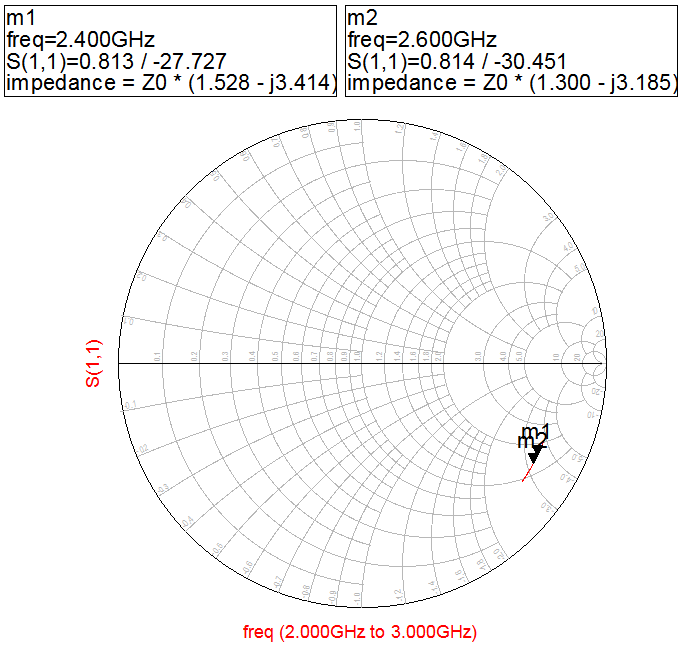
\includegraphics[scale=0.4]{diode-pics/diodedetectorSimplifiedSmithChart.png}
\caption{Smith chart plot of simple diode detector circuit with unmatched input.}
\label{fig:DDPlot}
\end{figure}

% Smith chart tool
\begin{figure}[!htb]
\centering
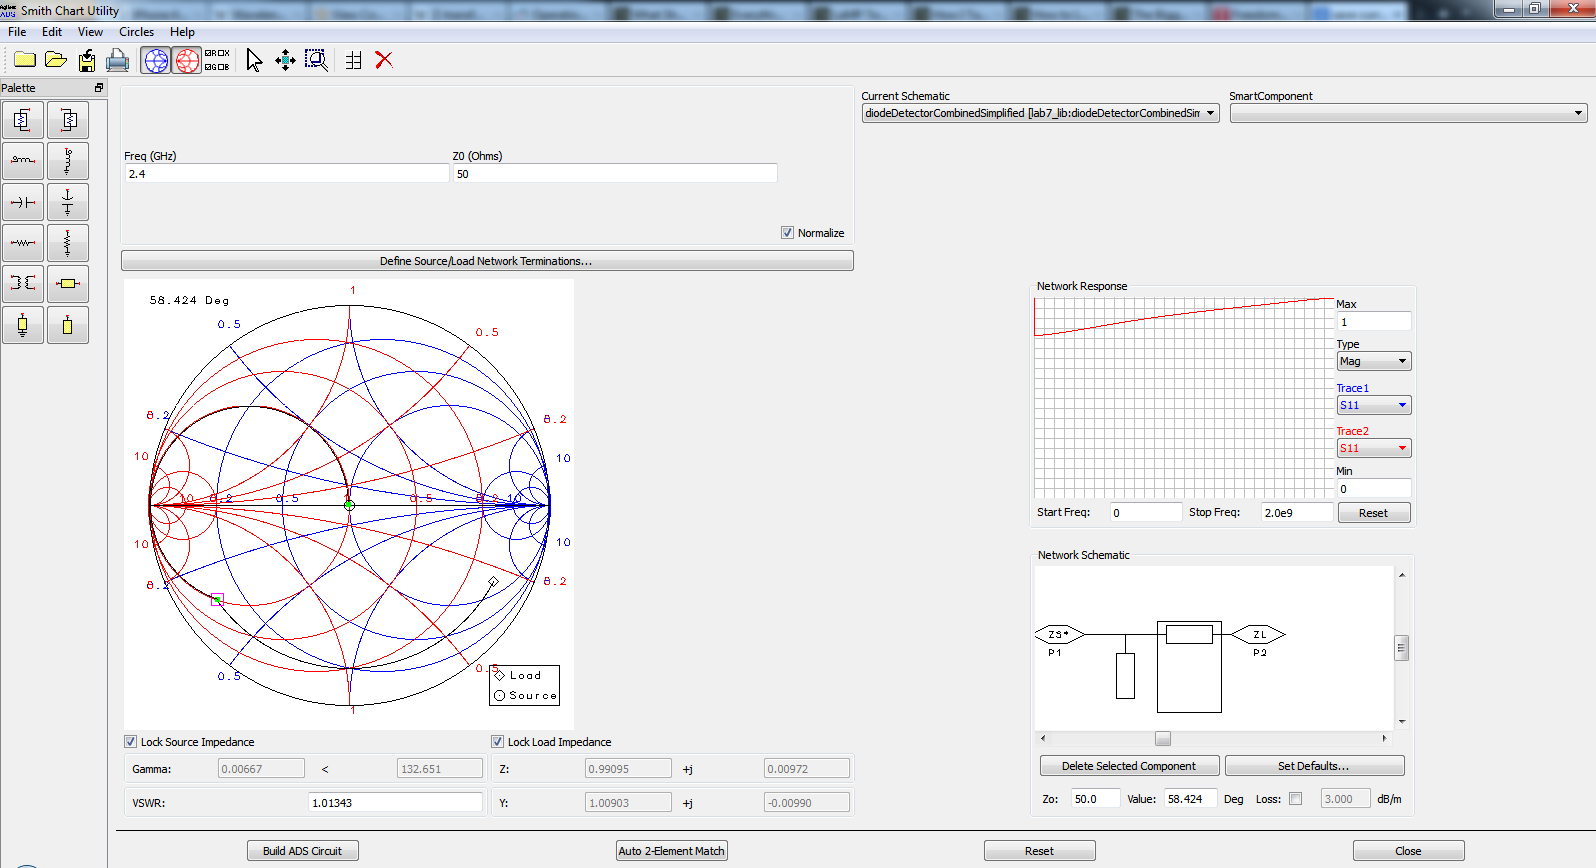
\includegraphics[scale=0.2]{diode-pics/smithcharttool.png}
\caption{ADS built-in Smith chart matching tool.}
\label{fig:smithchartTool}
\end{figure}

\begin{table}
   \caption{Final OC and microstrip lines for the 2.4 and 2.6 GHz diode detector circuits}
    \begin{tabular}{|l|l|l|l|l}
   \hline
    Parameter                          & 2.4 GHz    & 2.6 GHz  \\ \hline
    50 $\Omega$ Line (mm)       & 2.9131     & 2.9131   \\ \hline
    OC Stub Length (mm)         & 20.9706722 &    12.91 \\ \hline
    Microstrip Line Length (mm) & 7.1595414  & 11.97    \\ \hline
    \end{tabular}
\label{tab:diodetable}
\end{table}

% Final diode detector circuit schematic
\begin{figure}[!htb]
\centering
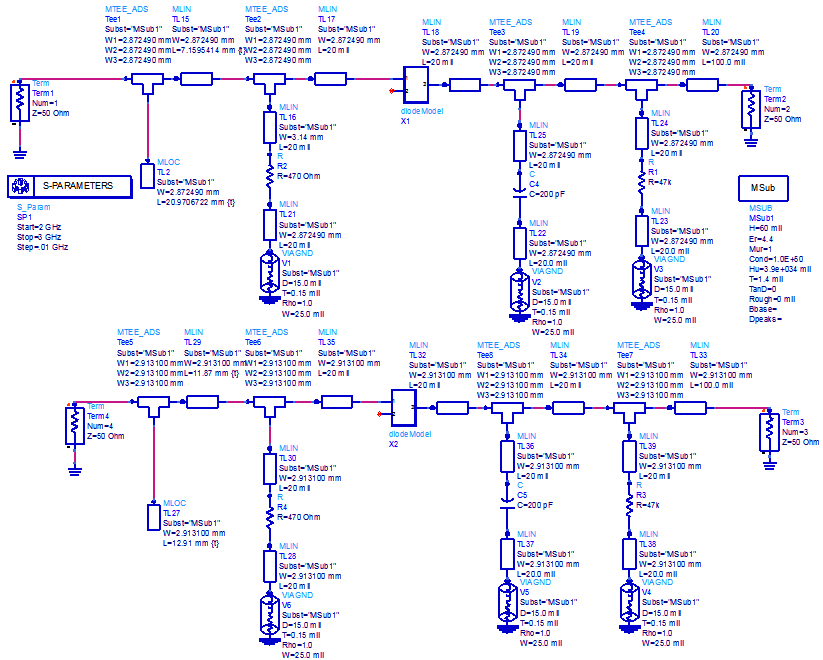
\includegraphics[scale=0.4]{diode-pics/diodedetectorsfinalchematic.png}
\caption{Complete diode detector circuit with properly matched input (2.4 GHz detector above and 2.6 GHz detector below).}
\label{fig:FinalDDSchematic}
\end{figure}

\section{Diode Detector Simulation}
Figure~\ref{fig:FinalDDSmith} shows the Smith chart of the final circuit.  The input matching network is verified to detect a signal at 2.4 GHz and 2.6 GHz.  Figure~\ref{fig:FinalDDS11} shows the S11 reflection.  The simulation results a narrow point at the matched frequency.  While the simulation shows impressive results, constructing the two circuits in the EPL will be very difficult due to manufacturing variations.  Thus, it is anticipated that the the center frequency will not be near 2.4 GHz and 2.6 GHz.

% Final diode detector circuit smith chart
\begin{figure}[!htb]
\centering
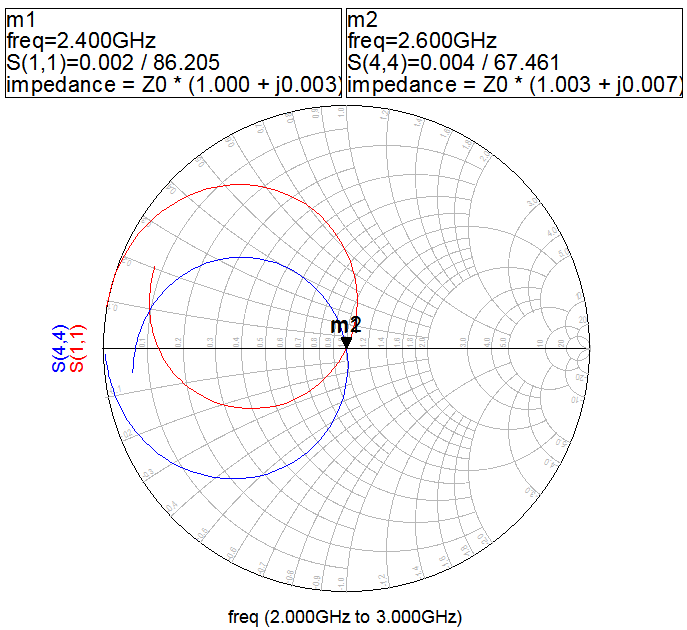
\includegraphics[scale=0.4]{diode-pics/diodedetectorSmithmatched-final.png}
\caption{Smith chart plot of complete diode detector circuit with properly matched input.}
\label{fig:FinalDDSmith}
\end{figure}

% Final diode detector circuit S11
\begin{figure}[!htb]
\centering
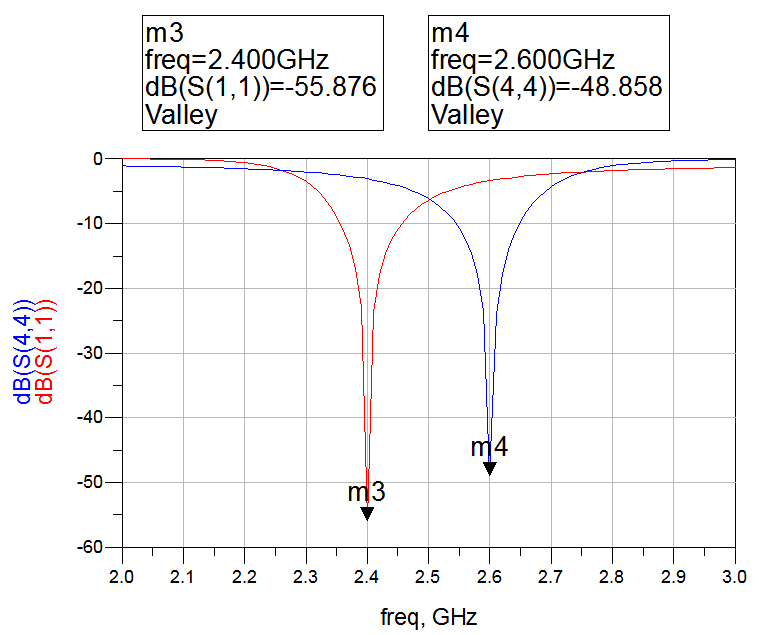
\includegraphics[scale=0.4]{diode-pics/diodedetectorS11matched-final.png}
\caption{S11 plot of complete diode detector circuit with properly matched input.}
\label{fig:FinalDDS11}
\end{figure}

% Diode detector layout
\begin{figure}[!htb]
\centering
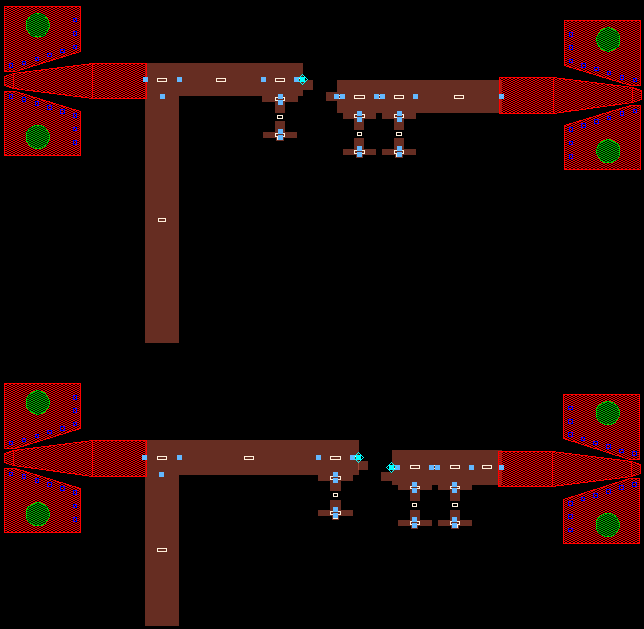
\includegraphics[scale=0.45]{diode-pics/diodedetectorlayout.png}
\caption{Layout of complete diode detector circuit with properly matched input (2.4 GHz detector above and 2.6 GHz detector below).}
\label{fig:FinalDDLayout}
\end{figure}

\section{Diode Detector Lab Results}
Figure~\ref{fig:FinalDDLayout} shows the diode detector layout.  The circuit was fabricated using the LPKF in the EPL.
\subsection{2.4 GHz Diode Detector}
Figure~\ref{fig:resultSmith24} shows a comparison between the simulation and the actual measurements in the lab.  The match did not work and will have significant signal loss.  This will be verified by looking at the S11 magnitude. Figure~\ref{fig:resultS1124} shows the S11 comparison.  The poor result from the lab will have a negative impact on the overall FSK receiver.
\subsection{2.6 GHz Diode Detector}
 Figure~\ref{fig:resultSmith26} shows a comparison between the simulation and the actual measurements in the lab.  The match is fairly close but the frequency sweep travels in a different direction than what ADS preditcs.  This may prove to be a worthwhile and interesting point to explore. Figure~\ref{fig:resultS1126} shows the S11 comparison.  The lab results are not as impressive as the simulation but still show that the circuit works well and is matched very close to 2.6 GHz.

% Diode detector 2.4 GHz circuit Smith chart Lab Result
\begin{figure}[!htb]
\centering
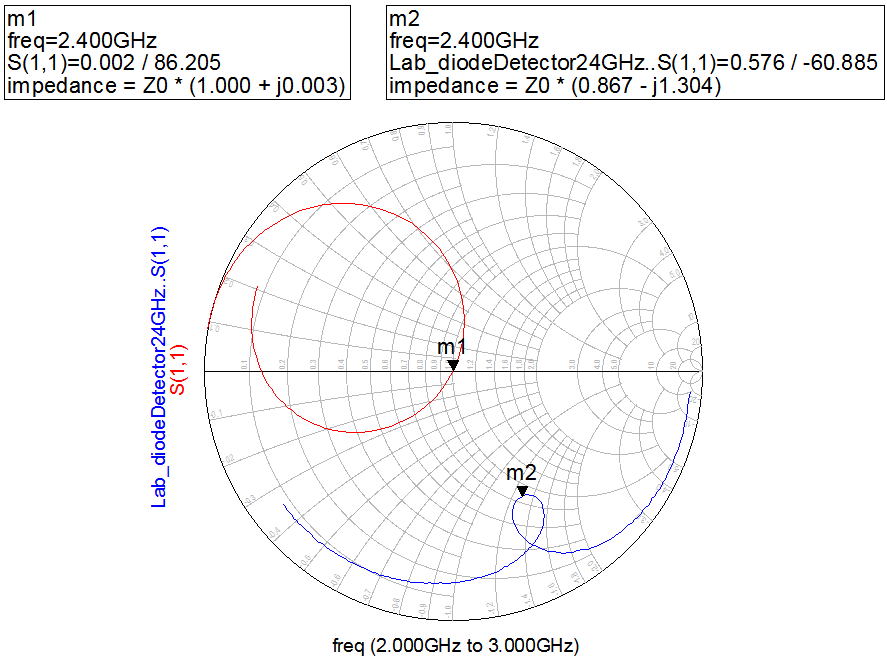
\includegraphics[scale=0.4]{diode-pics/diodedetectorLab24Smith.png}
\caption{Smith chart comparison between simulation and in-lab results for 2.4 GHz diode detector.}
\label{fig:resultSmith24}
\end{figure}

% Diode detector 2.4 GHz circuit S11 Lab Result
\begin{figure}[!htb]
\centering
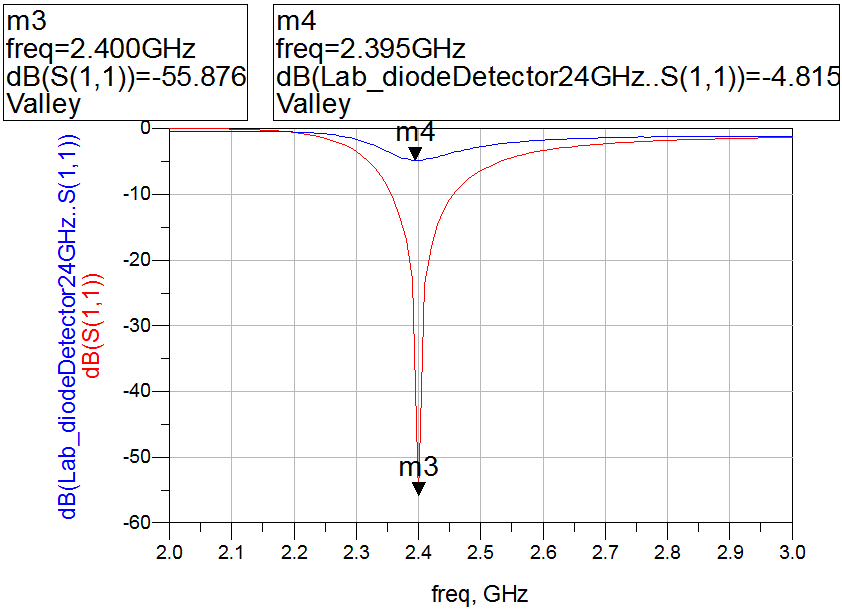
\includegraphics[scale=0.4]{diode-pics/diodedetectorLab24S11.png}
\caption{S11 plot comparison between simulation and in-lab results for 2.4 GHz diode detector.}
\label{fig:resultS1124}
\end{figure}

% Diode detector 2.6 GHz circuit Smith chart Lab Result
\begin{figure}[!htb]
\centering
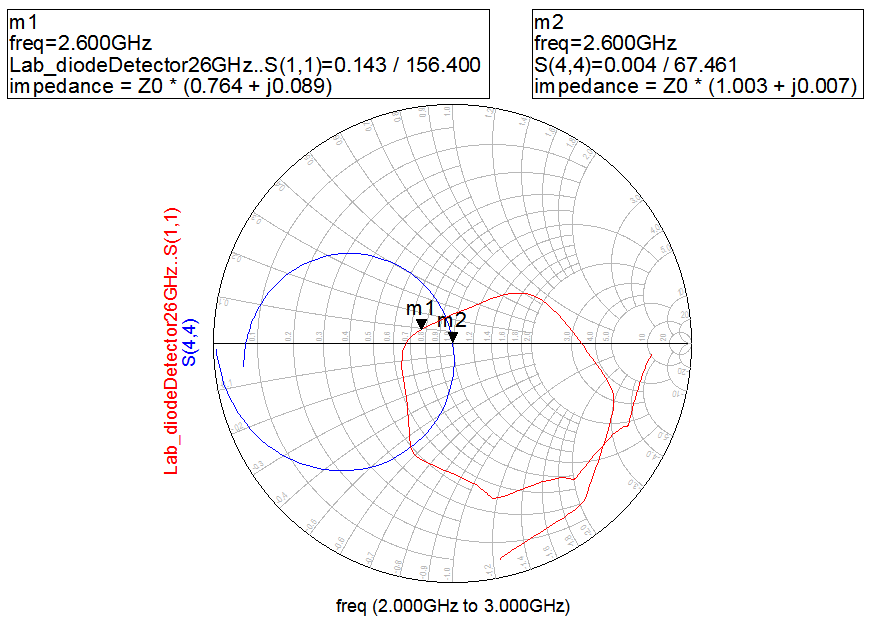
\includegraphics[scale=0.4]{diode-pics/diodedetectorLab26Smith.png}
\caption{Smith chart comparison between simulation and in-lab results for 2.6 GHz diode detector.}
\label{fig:resultSmith26}
\end{figure}

% Diode detector 2.6 GHz circuit S11 Lab Result
\begin{figure}[!htb]
\centering
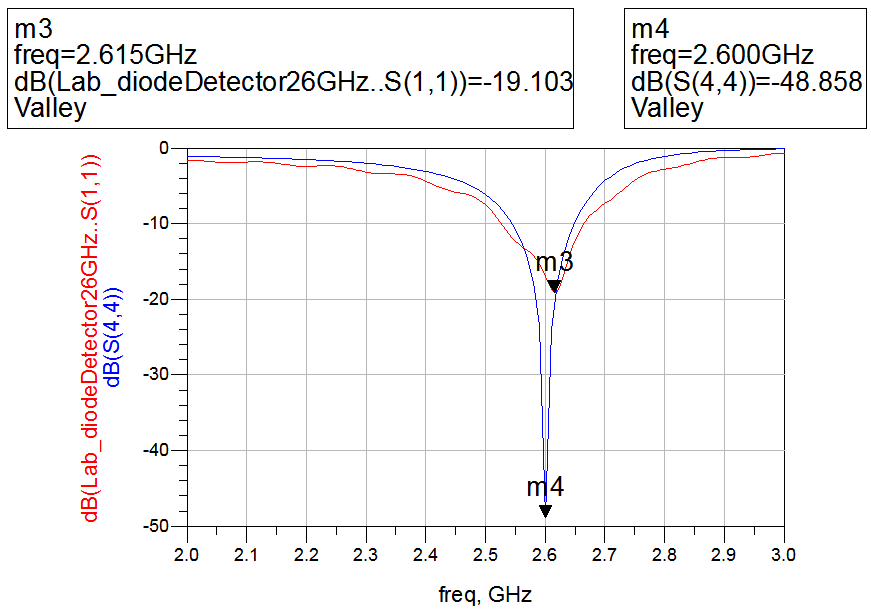
\includegraphics[scale=0.4]{diode-pics/diodedetectorLab26S11.png}
\caption{S11 plot comparison between simulation and in-lab results for 2.6 GHz diode detector.}
\label{fig:resultS1126}
\end{figure}

\section{FSK Receveiver Design}
The FSK receiver was built using the results from above and connecting the subcircuits together\footnote{Due to the lack of components, the entire FSK receiver was not built on a single PCB.}.  Figure~\ref{fig:fsk} shows the final FSK receiver.

% FSK Receiver
\begin{figure}[!htb]
\centering
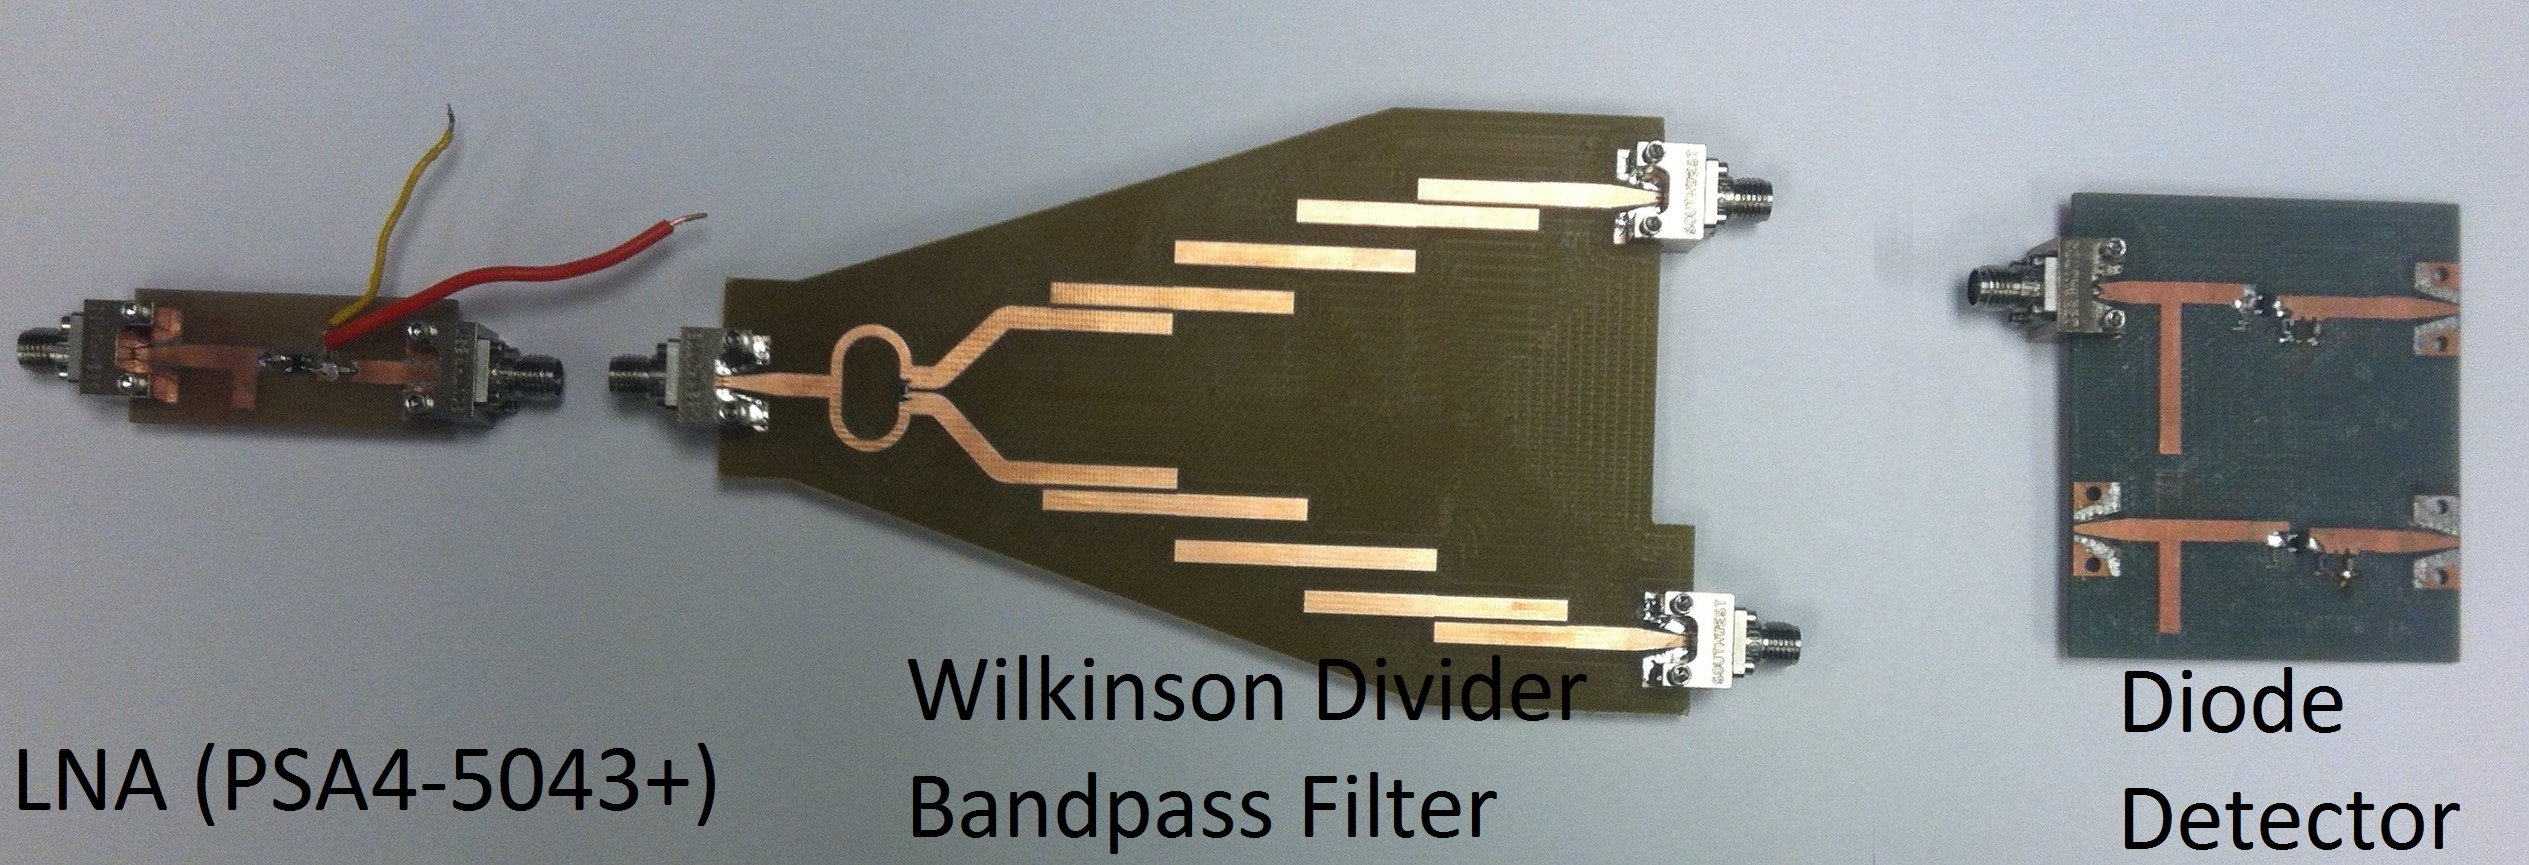
\includegraphics[scale=0.1]{fsk.jpg}
\caption{FSK receiver.}
\label{fig:fsk}
\end{figure}

\section{FSK Receveiver Lab Results}
Table~\ref{tab:fsk24} and Table~\ref{tab:fsk26} show the measured results obtained from the FSK receiver.  The main problems in the design stem from the bandpass filter being off by 100 MHz as well as the mismatch on the diode detector.  Improving these two circuits will yield better results.

\begin{table}
\caption{FSK Receiver 2.4 GHz Frequency Sweep}
    \begin{tabular}{|l|l|}
    \hline
    Frequency Sweep (GHz) & Output Signal at 0 dBm (mV) \\\hline
    2.25                  & 124                         \\\hline
    2.30                  & 320                         \\\hline
    2.35                  & 290                         \\\hline
    2.40                  & 40                          \\\hline
    2.45                  & 4                           \\\hline
    2.50                  & 0.56                        \\\hline
    2.55                  & 0.08                        \\\hline
    2.60                  & 1.2                         \\\hline
    \end{tabular}
\label{tab:fsk24}
\end{table}

\begin{table}
\caption{FSK Receiver 2.6 GHz Frequency Sweep}
    \begin{tabular}{|l|l|}
    \hline
    Frequency Sweep (GHz) & Output Signal at 0 dBm (mV) \\ \hline
    2.30                  & 4                           \\ \hline
    2.35                  & 44                          \\ \hline
    2.40                  & 430                         \\ \hline
    2.45                  & 950                         \\ \hline
    2.50                  & 1100                        \\ \hline
    2.55                  & 800                         \\\hline
    2.60                  & 110                         \\ \hline
    2.65                  & 80                          \\\hline
    2.70                  & 1.3                         \\\hline
    \end{tabular}
\label{tab:fsk26}
\end{table}

% Bibliography
\begin{thebibliography}{1}
\bibitem{an1124}
Avago Application Note 1124
\bibitem{payne}
K. Payne, "Practical RF Amplifier Design Using the Available Gain Procedure and the Advanced Design System EM/Circuit Co-Simulation Capability," Agilent Technologies (5990-3356EN), 2008.
\bibitem{lunan}
Zhang, Lunan, ECE 532/432 Microwave Circuit Design II Lab TA
\end{thebibliography}
\end{document}